\subsection{Controlador PID}

Baseando-se nas análises realizadas na Atividade 4, foi possível determinar um valor limite para o ganho crítico \( K_c \) de 14.93. Esta descoberta é essencial para o ajuste dos parâmetros do controlador PID segundo o método de Ziegler-Nichols.
Além como na atividade 5, tenhamos que simular o comportamento do sistema usando como entrada um sinal degrau de amplitude A= m/4, para nosso caso m=10, iremos A=10/4=2.5, logo iremos ter o diagrama com ganho  para  

\begin{figure}[H]
    \centering
    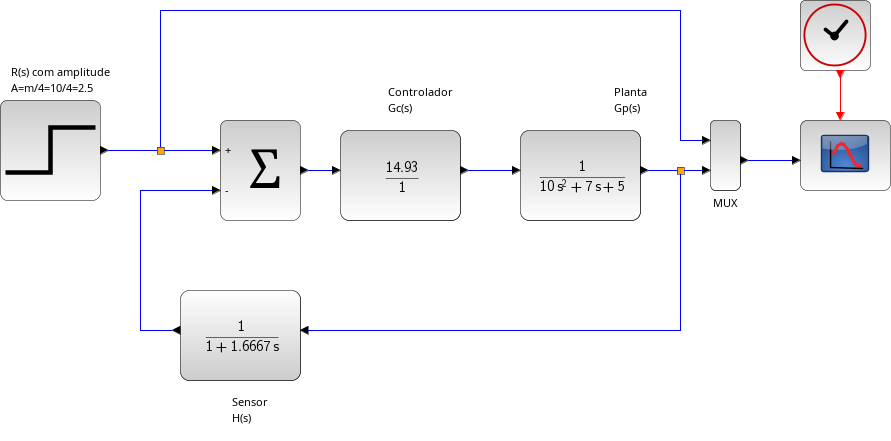
\includegraphics[width=0.7\textwidth]{6-atividade/assets/a/diagrama-ganho-critico-sistema-instavel.png}
    \caption{Diagrama mostrando o sistema no ponto crítico com \( K_c = 14.93 \)}
    \label{fig:diagrama-ponto-critico}
\end{figure}

A simulação realizada com \( K_c = 14.93 \) demonstrou que o sistema alcança um estado crítico, como evidenciado no gráfico abaixo:

\begin{figure}[H]
    \centering
    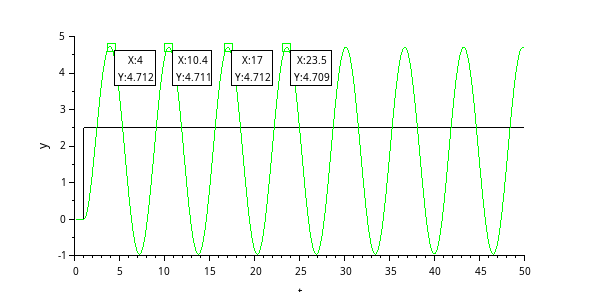
\includegraphics[width=0.7\textwidth]{6-atividade/assets/a/ganho-critico-sistema-instavel.png}
    \caption{Resposta do sistema com o controlador PID ajustado para \( K_c = 14.93 \)}
    \label{fig:ganho-critico-sistema-instavel}
\end{figure}



A resposta simulada revela claramente o comportamento do sistema na condição de ganho crítico, possibilitando a utilização desses dados para calibrar os parâmetros do controlador PID, garantindo eficiência e estabilidade no controle do sistema.

\subsubsection{Determinação do Período Crítico}
O período crítico \( P_c \) foi determinado a partir da análise do gráfico de resposta em regime oscilatório no ganho crítico. Identificamos os picos consecutivos e medimos o tempo entre eles para calcular o \( P_c \). A partir dos pontos identificados no gráfico, com os tempos \( t_1 = 9.98 \, \text{s} \) e \( t_2 = 16.894 \, \text{s} \), o período crítico foi calculado como:
\[
    P_c = t_2 - t_1 = 16.894 - 10.452 = 6,442 \, \text{s}
\]
Este valor é crucial para o ajuste subsequente dos parâmetros do controlador PID utilizando o método de Ziegler-Nichols.


\subsubsection{Determinação dos Parâmetros do Controlador PID}
Após identificarmos o ganho crítico \( K_c = 14.93 \) através de análises detalhadas, empregamos o método de Ziegler-Nichols para ajustar os parâmetros do controlador PID. Este método é eficaz para sintonizar controladores em sistemas onde a resposta precisa ser otimizada em termos de estabilidade e rapidez.

\subsubsection{Cálculo dos Parâmetros do Controlador PID}
O método de Ziegler-Nichols, conhecido por sua eficiência na configuração inicial de controladores PID, utiliza o ganho crítico \( K_c \) e o período crítico \( P_c \) para estabelecer os parâmetros de controle, ajustando assim a resposta do sistema.

\begin{itemize}
    \item \textbf{Ganho Proporcional} \( K_p \):
          \[
              K_p = 0.6 \times K_c = 0.6 \times 14.93 \approx 8.958
          \]
    \item \textbf{Ganho Integral} \( K_i \):
          \[
              K_i = \frac{2}{P_c} = \frac{2}{6,442} \approx 0.310462589
          \]
    \item \textbf{Ganho Derivativo} \( K_d \):
          \[
              K_d = 0.125 \times P_c = 0.125 \times 6,442 = 0.80525
          \]
\end{itemize}

\subsubsection{Implementação e Validação dos Parâmetros}
Os parâmetros \( K_p = 8.958 \), \( K_i = 0.310462589 \), e \( K_d = 0.80525 \) são implementados no controlador PID no ambiente de simulação, como Scilab. Esses valores são projetados para ajustar o sistema para responder de forma ideal em várias condições operacionais, melhorando a estabilidade e precisão do sistema.

A eficácia desses parâmetros será validada por meio de simulações subsequentes, as quais confirmarão se eles mantêm o desempenho desejado do sistema, garantindo que o controle PID seja tanto eficiente quanto efetivo.

\begin{figure}[H]
    \centering
    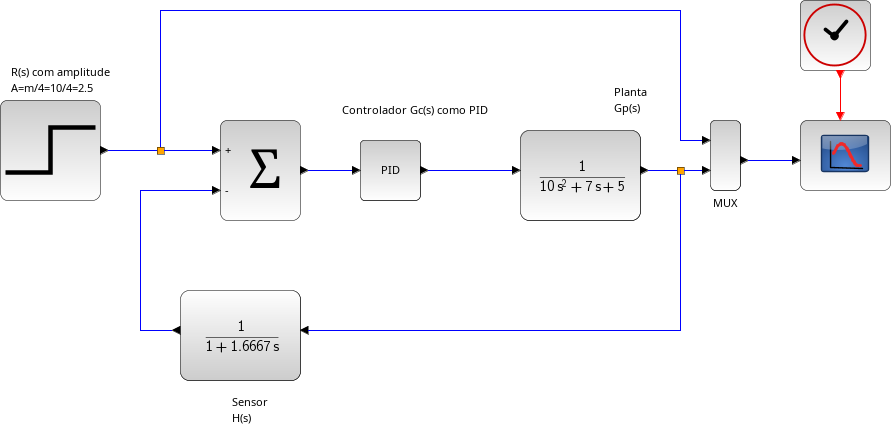
\includegraphics[width=0.8\textwidth]{6-atividade/assets/a/diagrama-pid.png}
    \caption{Resposta do sistema com os parâmetros do PID ajustados.}
    \label{fig:diagrama-pid}
\end{figure}

\begin{figure}[H]
    \centering
    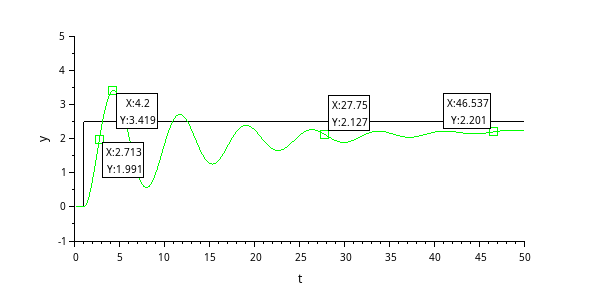
\includegraphics[width=0.8\textwidth]{6-atividade/assets/a/pid.png}
    \caption{Resposta do sistema com os parâmetros do PID ajustados.}
    \label{fig:resposta-pid}
\end{figure}

Após a validação inicial, um refinamento manual dos parâmetros pode ser necessário para otimizar ainda mais a resposta do sistema. Este processo de ajuste fino baseia-se na análise das respostas obtidas e na experiência prática, permitindo uma sintonia mais precisa que responde de maneira adequada às especificidades do sistema e às variações nas condições operacionais. Este ajuste fino é crucial para alcançar a melhor performance, equilibrando a estabilidade e a rapidez da resposta do controlador PID.

Subsequentemente, novas simulações serão realizadas para validar a eficácia dos parâmetros ajustados. Essa etapa é crucial para verificar se os ajustes refinados mantêm a saída do sistema próxima ao valor desejado sob uma gama mais ampla de condições operacionais, garantindo a eficácia e a eficiência do controlador.
